\documentclass[a4,12pt]{horizon-theme}
\usepackage{lipsum}
\usepackage{fontawesome5}
\usepackage{graphicx,url}
\usepackage{float}
\usepackage{amsmath}
\usepackage{booktabs}
\usepackage{makecell}
\usepackage{array}
\usepackage{multirow}
\usepackage{caption}
\usepackage{subcaption}
\usepackage{siunitx}
\usepackage{enumerate}
\usepackage{gensymb}
\usepackage{csvsimple}
% \usepackage{tabularray}
\usepackage{stackengine}
\usepackage{xcolor, colortbl}
\usepackage[round]{natbib}
\usepackage{karnaugh-map}
\usepackage{stackengine}
% \usepackage{longtable}

\strutlongstacks{T}


% Cover Config
% \configCover{<num. do exp.>}{<data>}{<título>}
\configCover{4}{28/04/2022}{Projeto de Contadores Síncronos Usando Flip-Flops e CI 74LS163}


\begin{filecontents*}{tb_verdade_ff.csv}
clk,clr,Q3,Q2,Q1,Q0,D3,D2,D1,D0
-,0,0,0,0,0,0,0,0,1
$\uparrow$,1,0,0,0,0,0,0,0,1
$\uparrow$,1,0,0,0,1,0,0,1,0
$\uparrow$,1,0,0,1,0,0,0,1,1
$\uparrow$,1,0,0,1,1,0,1,0,0
$\uparrow$,1,0,1,0,0,0,1,0,1
$\uparrow$,1,0,1,0,1,0,1,1,0
$\uparrow$,1,0,1,1,0,0,1,1,1
$\uparrow$,1,0,1,1,1,1,0,0,0
$\uparrow$,1,1,0,0,0,1,0,0,1
$\uparrow$,1,1,0,0,1,1,0,1,0
$\uparrow$,1,1,0,1,0,0,0,0,0
$\uparrow$,1,1,0,1,1,-,-,-,-
$\uparrow$,1,1,1,0,0,-,-,-,-
$\uparrow$,1,1,1,0,1,-,-,-,-
$\uparrow$,1,1,1,1,0,-,-,-,-
$\uparrow$,1,1,1,1,1,-,-,-,-
\end{filecontents*}

\begin{filecontents*}{tb_teste_ff.csv}
clk,clr,Q3,Q2,Q1,Q0,D3,D2,D1,D0,Q3,Q2,Q1,Q0,D3,D2,D1,D0
-,0,0,0,0,0,0,0,0,1,0,0,0,0,0,0,\bf{1},1
$\uparrow$,1,0,0,0,0,0,0,0,1,0,0,0,0,0,0,\bf{1},1
$\uparrow$,1,0,0,0,1,0,0,1,0,-,-,-,-,-,-,-,-
$\uparrow$,1,0,0,1,0,0,0,1,1,-,-,-,-,-,-,-,-
$\uparrow$,1,0,0,1,1,0,1,0,0,0,0,1,1,0,1,0,0
$\uparrow$,1,0,1,0,0,0,1,0,1,0,1,0,0,0,1,1,1
$\uparrow$,1,0,1,0,1,0,1,1,0,-,-,-,-,-,-,-,-
$\uparrow$,1,0,1,1,0,0,1,1,1,-,-,-,-,-,-,-,-
$\uparrow$,1,0,1,1,1,1,0,0,0,0,1,1,1,1,0,0,0
$\uparrow$,1,1,0,0,0,1,0,0,1,1,0,0,0,1,0,0,1
$\uparrow$,1,1,0,0,1,1,0,1,0,1,0,0,1,1,0,1,0
$\uparrow$,1,1,0,1,0,0,0,0,0,1,0,1,0,0,0,0,0
$\uparrow$,1,1,0,1,1,-,-,-,-,1,0,1,1,-,-,-,-
$\uparrow$,1,1,1,0,0,-,-,-,-,1,1,0,0,-,-,-,-
$\uparrow$,1,1,1,0,1,-,-,-,-,1,1,0,1,-,-,-,-
$\uparrow$,1,1,1,1,0,-,-,-,-,1,1,1,0,-,-,-,-
$\uparrow$,1,1,1,1,1,-,-,-,-,1,1,1,1,-,-,-,-
\end{filecontents*}

\begin{filecontents*}{tb_verdade_74163.csv}
clk,QD,QC,QB,QA,Z,clr,load
$\uparrow$,0,0,0,0,0,1,1
$\uparrow$,0,0,0,1,0,1,1
$\uparrow$,0,0,1,0,0,1,1
$\uparrow$,0,0,1,1,0,1,1
$\uparrow$,0,1,0,0,0,1,1
$\uparrow$,0,1,0,1,0,1,1
$\uparrow$,0,1,1,0,0,1,1
$\uparrow$,0,1,1,1,0,1,1
$\uparrow$,1,0,0,0,0,1,1
$\uparrow$,1,0,0,1,0,1,1
$\uparrow$,1,0,1,0,1,0,0
$\uparrow$,1,0,1,1,1,0,0
$\uparrow$,1,1,0,0,1,0,0
$\uparrow$,1,1,0,1,1,0,0
$\uparrow$,1,1,1,0,1,0,0
$\uparrow$,1,1,1,1,1,0,0
\end{filecontents*}

\begin{filecontents*}{tb_teste_74163.csv}
clk,QD,QC,QB,QA,Z
$\uparrow$,0,0,0,0,0
$\uparrow$,0,0,0,1,0
$\uparrow$,0,0,1,0,0
$\uparrow$,0,0,1,1,0
$\uparrow$,0,1,0,0,0
$\uparrow$,0,1,0,1,0
$\uparrow$,0,1,1,0,0
$\uparrow$,0,1,1,1,0
$\uparrow$,1,0,0,0,0
$\uparrow$,1,0,0,1,0
$\uparrow$,1,0,1,0,1
\end{filecontents*}


\begin{filecontents*}{vcc1.csv}
pos,comp,vcc,gnd
FF1,7474,14,7
FF2,7474,14,7
\end{filecontents*}


\begin{filecontents*}{vcc2.csv}
pos,comp,vcc,gnd
C1,7408,14,7
C2,7408,14,7
C3,7432,14,7
C4,7408,14,7
C5,7411,14,7
C6,7432,14,7
C7,7408,14,7
C8,7408,14,7
C9,7432,14,7
C10,7411,14,7
C11,7408,14,7
C12,7432,14,7
C13,7408,14,7
C14,7411,14,7
C15,7432,14,7
\end{filecontents*}


\begin{filecontents*}{vcc3.csv}
pos,comp,vcc,gnd
C1,74LS163,16,8
C2,7404,14,7
C3,7432,14,7
C4,7408,14,7
\end{filecontents*}


\begin{document}
\horizonCover

\horizonTitle


\section{Introdução} % R

Circuitos lógicos são divididos em dois tipos, circuitos lógicos combinatórios e circuitos lógicos sequenciais. Os cirucuitos lógicos combinatórios são aqueles que a saída depende exclusivamente das entradas atuais. Já um circuito lógico sequencial depende não apenas das entradas atuais como também da sequencia de entradas passadas, que, possivelmente, são bem anteriores ao momento atual da entrada.

Como em alguns projetos de circuitos digitais a quantidade de entradas passadas é muito grande para serem todas armazenadas, é utilizada uma variável de estado que determina o estado atual do circuito. E, é com essa variável de estado que os circuito lógicos sequencias trabalhão. Ou seja, a saída de um circuito lógico sequencial depende apenas da entrada atual e de seu estado atual.

\section{Objetivos} % N
O objetivo deste experimento é projetar e construir dois circuitos contadores síncronos de módulo 11, um usando flip-flops tipo D (Seção \ref{sec:plan_ff}) e outro usando o CI 74LS163 (Seção \ref{sec:plan_74163}), ambos com contagem de $(0)_{10}$ a $(10)_{10}$.


\section{Planejamento} % N, R
\label{sec:plan}

\subsection{Contador usando flip-flops}
\label{sec:plan_ff}

A Fig. \ref{fig:diagrama_blocos_ff} mostra o diagrama de blocos do contador que será projetado usando flip-flops tipo D. O circuito é dividido em dois blocos: os flip-flops e o circuito de próximo estado. O primeiro bloco é um conjunto de dois dispositivos TTL 7474, cada um com dois flip-flops tipo D. Estes dispositivos recebem o mesmo sinal de clock (\texttt{CLK}) e reset (\texttt{CLR}). Isto é, o clock é sincrono para todos os flip-flops, mas o reset é assíncrono em relação ao clock. E o segundo bloco é um circuito combinatório que tem o objetivo de calcular o próximo estado dos flip-flops a partir do estado atual. A saída do circuito são as saídas não-invertidas dos flip-flops (\texttt{Q}).

\begin{figure}[!ht]
  \centering
  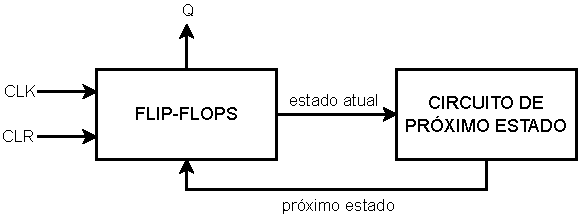
\includegraphics[width=0.81\textwidth]{diagrama_blocos_ff.pdf}
  \caption{Diagrama de blocos do circuito contador síncrono usando flip-flops}
  \label{fig:diagrama_blocos_ff}
\end{figure}



\subsubsection{Síntese do Circuito de Próximo Estado}
\label{sec:plan_ff_uc}

\begin{table}[!ht]
  \centering
  \caption{Tabela Verdade com os valores de entrada, valore de saída dos flip-flops e valores de saída do circuito de próximo estado, que é o valor do próximo estado}
  \label{tab:tb_verdade_ff}
  \doubleRuleSep
  \begin{tabular}{*{10}{c}}
    \doubleTopRule
    \multicolumn{2}{c}{Entrada} & \multicolumn{4}{c}{Saída FF} & \multicolumn{4}{c}{Saída CPE}                                                                                       \\
    \cmidrule(lr){1-2}\cmidrule(lr){3-6}\cmidrule(lr){7-10}
    clk                         & clr                          & $Q_3$                         & $Q_2$     & $Q_1$    & $Q_0$     & $D_3$      & $D_2$       & $D_1$     & $D_0$     \\
    \midrule
    \csvreader[head to column names, late after line=\\]{tb_verdade_ff.csv}{}%
    {\csvcoli                   & \csvcolii                    & \csvcoliii                    & \csvcoliv & \csvcolv & \csvcolvi & \csvcolvii & \csvcolviii & \csvcolix & \csvcolx} %
    \doubleBottomRule
  \end{tabular}
\end{table}

A síntese do circuito de próximo estado constitui na construção de um circuito que calcule o próximo estado dos flip-flops a partir do estado atual seguindo a tabela verdade descrita na Tabela \ref{tab:tb_verdade_ff}. Esta tabela mostra a lógica de um contador de módulo 11 sensível à borda de subida do clock (síncrono) e um reset assíncrono (primeira linha da tabela). As colunas clk e clr representam os sinais de entrada, clock e reset, respectivamente, as colunas $Q_3$, $Q_2$, $Q_1$ e $Q_0$ representam as saídas não-invertidos de cada um dos flip-flops, o flip-flop 3 foi adotado como mais significativo, e, por fim, as colunas $D_3$, $D_2$, $D_1$ e $D_0$ representam as saída do circuito de próximo estado para o respectivo flip-flop com o valor do próximo estado. As saídas não-invertidas dos flip-flops são as saídas do contador, enquanto que as saídas dao circuito de próximo estado têm caráter de depuração apenas. A partir desta tabela, são feitos os mapas de Karnaugh para cada saída $D_i$ do circuito de próximo estado na Fig. \ref{fig:karnaugh_ff} no Apêndice \ref{ap:ff_karnaugh}. Com isso, foram obtidas as expressões lógicas para cada saída do circuito de próximo estado nas eqs. \eqref{eq:ff_d0}, \eqref{eq:ff_d1}, \eqref{eq:ff_d2} e \eqref{eq:ff_d3}.

\begin{align}
  D_0 & = \n{Q_3} \cdot \n{Q_0} + \n{Q_1} \cdot \n{Q_0}\label{eq:ff_d0}                                     \\
  D_1 & = \n{Q_1} \cdot Q_0 + \n{Q_3} \cdot Q_1 \cdot \n{Q_0}\label{eq:ff_d1}                               \\
  D_2 & = Q_2 \cdot \n{Q_1} + Q_2 \cdot \n{Q_0} + \n{Q_3} \cdot \n{Q_2} \cdot Q_1 \cdot Q_0\label{eq:ff_d2} \\
  D_3 & = Q_3 \cdot \n{Q_1} + Q_2 \cdot Q_1 \cdot Q_0\label{eq:ff_d3}
\end{align}




\subsubsection{Diagrama lógico}
\label{sec:plan_ff_logico}

A Fig. \ref{fig:diagrama_logico_ff} mostra o diagrama lógico do contador síncrono. Ele é constituído de três componentes, dois físicos (CI's 7474) e um virtual (Circuito de Próximo Estado). O circuito de próximo estado, cujo diagrama lógico é mostrado na Fig. \ref{fig:diagrama_logico_uc}, é um circuito combinatório sintetizado a partir das eqs. \eqref{eq:ff_d0}, \eqref{eq:ff_d1}, \eqref{eq:ff_d2} e \eqref{eq:ff_d3}. Ela rebece todas as saídas, invertidas e não invertidas, dos flip-flops como entrada e define os valores do próximo estado, que são as entradas $D_i$ dos flip-flops.

\begin{figure}[!ht]
  \centering
  \stackinset{r}{1pt}{b}{1pt}{\carimboA{Contador FF}}{%
    \stackinset{l}{1pt}{b}{1pt}{\carimboB{vcc1.csv}}{%
      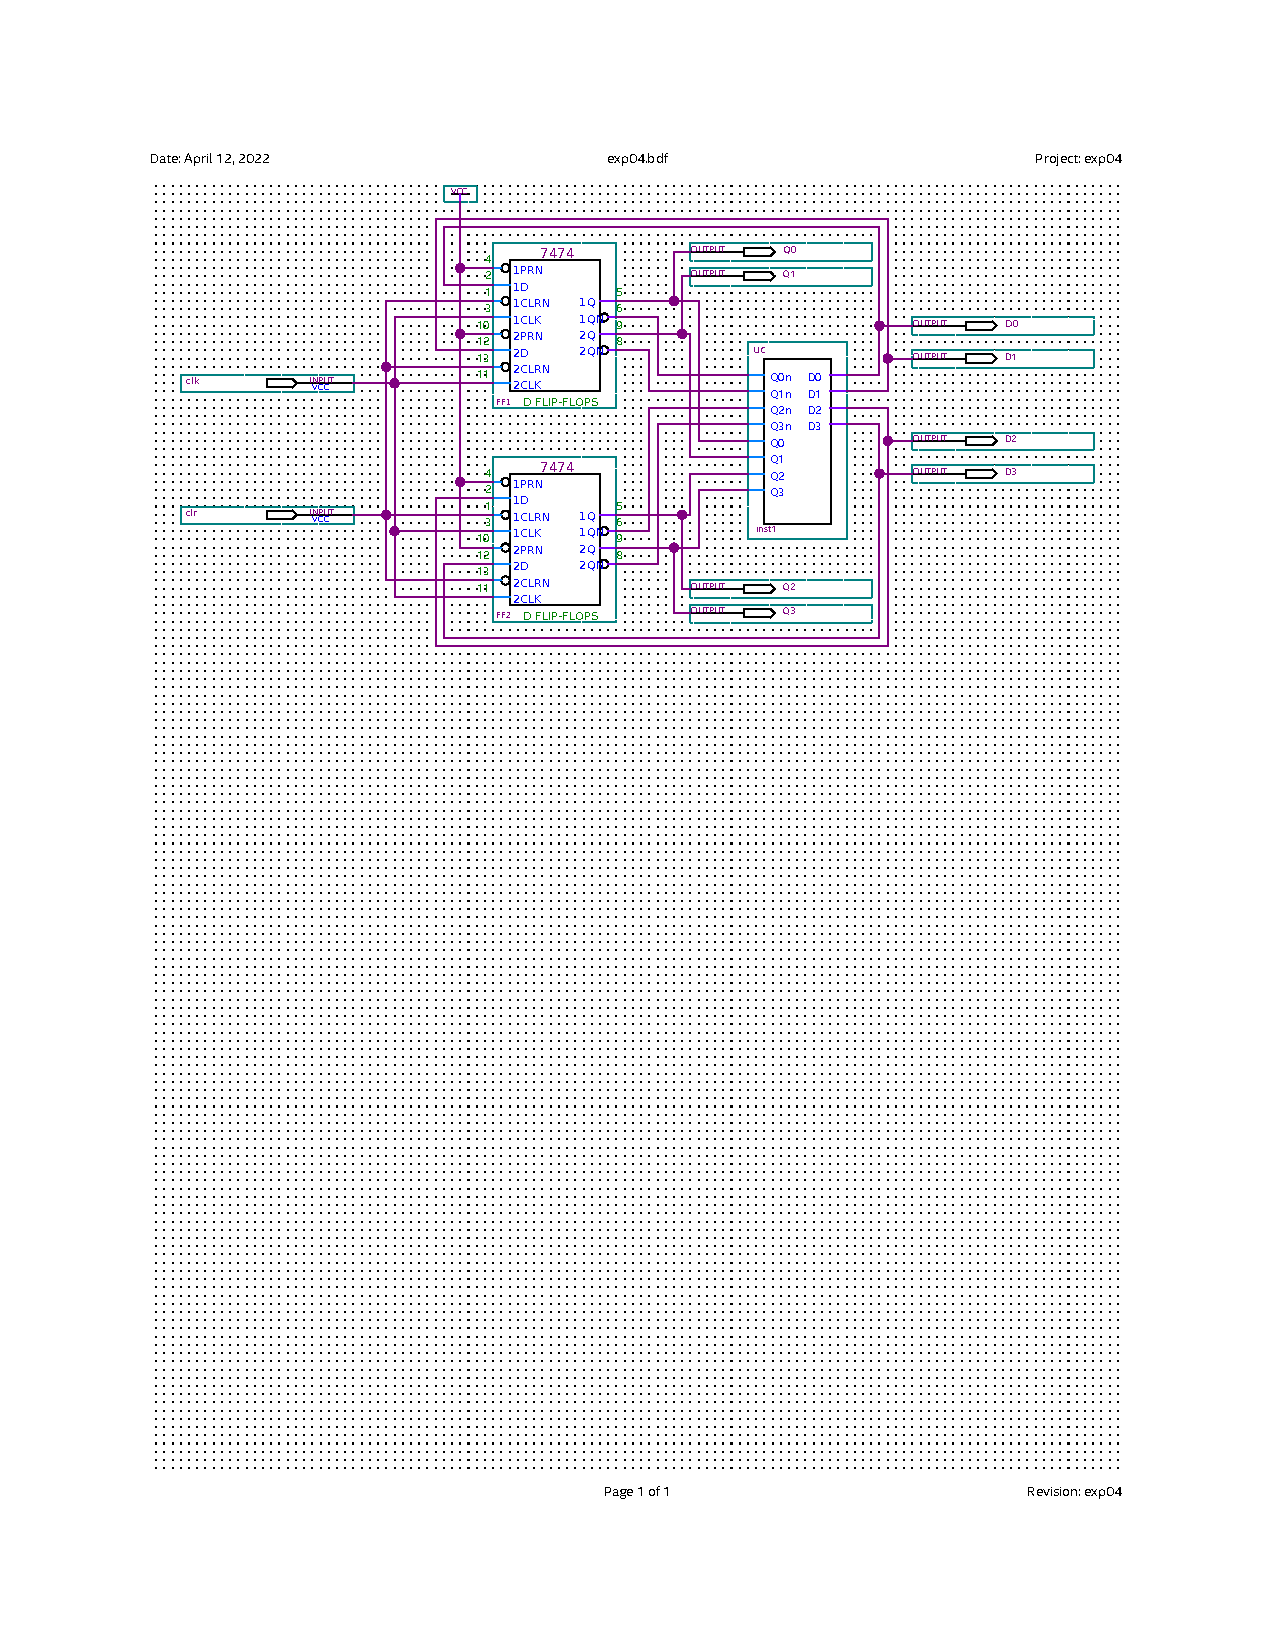
\includegraphics[width=\textwidth, trim={30mm, 148mm, 30mm, 30mm}, clip]{diagrama_ff}%
    }%
  }
  \caption{Diagrama lógico do contador usando dois flip-flops tipo D.}
  \label{fig:diagrama_logico_ff}
\end{figure}

\begin{figure}[!ht]
  \centering
  \stackinset{r}{1pt}{t}{1pt}{\carimboA{Contador FF (CPE)}}{%
    \stackinset{l}{1pt}{b}{1pt}{\carimboB{vcc2.csv}}{%
      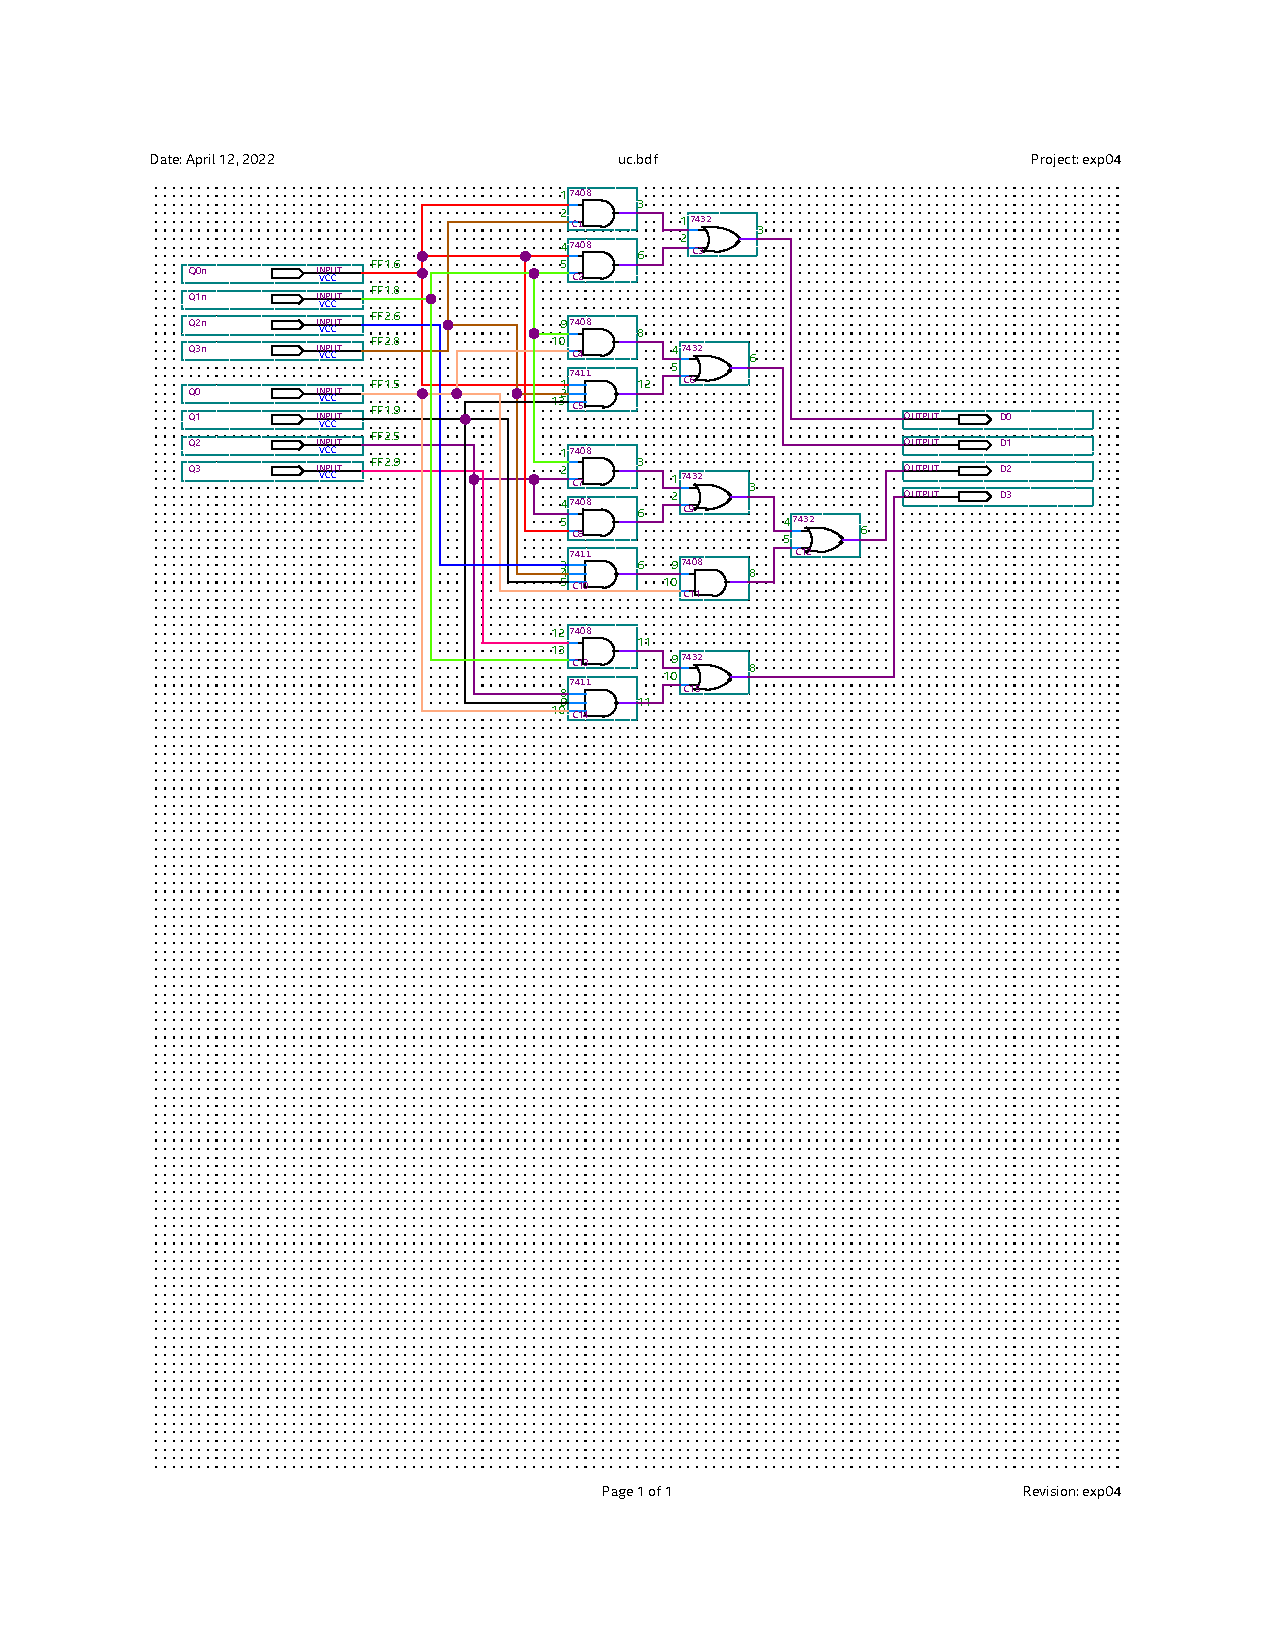
\includegraphics[width=\textwidth, trim={30mm, 156mm, 29mm, 31mm}, clip]{diagrama_uc}%
    }%
  }
  \caption{Diagrama lógico do circuito de próximo estado}
  \label{fig:diagrama_logico_uc}
\end{figure}


\newpage
\subsubsection{Levantamento dos materiais necessários}
\label{sec:plan_ff_materiais}


\begin{table}[!ht]
  \centering
  \caption{Unidades requeridas para cada CI}
  \label{tab:ff_materiais}
  \doubleRuleSep
  \begin{tabular}{lllrr}
    \doubleTopRule
    Slot & Operação & CI   & Un. Requeridas & Un. Disponíveis \\
    \midrule
    1    & FF       & 7474 & 2              & 2               \\
    2    & FF       & 7474 & 2              & 2               \\
    3    & AND2     & 7408 & 3              & 4               \\
    4    & OR2      & 7432 & 2              & 4               \\
    5    & AND3     & 7411 & 3              & 3               \\
    6    & AND2     & 7408 & 4              & 4               \\
    7    & OR2      & 7432 & 3              & 4               \\
    \doubleBottomRule
  \end{tabular}
\end{table}

Para garantir que o circuito projetado respeite as restrições de montagem, fizemos um levantamento dos recursos necessários para este circuito mostrado na Tabela \ref{tab:ff_materiais}. Ela mostra a quantidade de unidades lógicas requeridas para cada CI utilizado. As especificações de cada CI foi obtido pelos respectivos \emph{datasheets}.


\subsubsection{Simulação}
\label{sec:plan_ff_sim}

A Fig. \ref{sec:plan_ff_sim} mostra a carta dos tempos obtida com a simulação do contador. É possível notar que ela segue a tabela verdade descrita na Tabela \ref{tab:tb_verdade_ff}.

\begin{figure}[!ht]
  \centering
  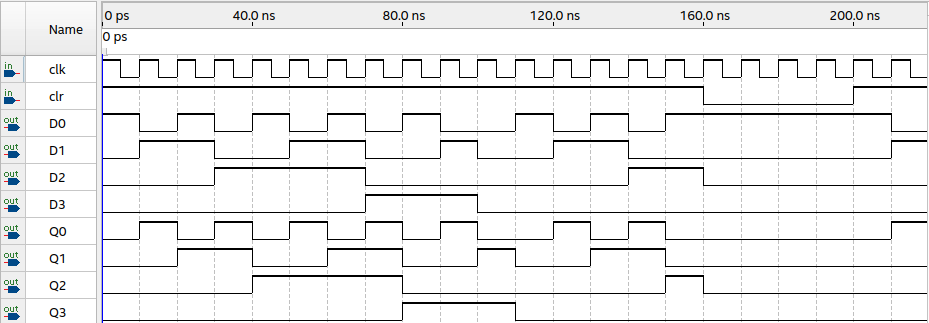
\includegraphics[width=\textwidth]{carta_tempos_ff.png}
  \caption{Carta dos tempos para o circuito contruído com flip-flops com sinias de entrada \texttt{clk} e \texttt{clr}, sinais de depuração $D_0$, $D_1$, $D_2$ e $D_3$ (saídas do circuito de próximo estado) e sinais de saída $Q_0$, $Q_1$, $Q_2$ e $Q_3$ (saídas dos flip-flops)}
  \label{fig:carta_tempos_ff}
\end{figure}


\subsubsection{Metodologia de montagem e testes}
\label{sec:plan_ff_montagem}

O circuito de próximo estado será construída separadamente dos flip-flops. Durante a construção, os valores de saída do circuito de próximo estado será comparada com os valores das colunas ``Saída UC'' da Tabela \ref{tab:tb_verdade_ff} e as entradas serão fornecidas diretamente pelo testador, e não pelos flip-flops. Analogamente, os flip-flops também serão construídos separadamente do circuito de próximo estado e receberão sinais de entrada diretamente do testador. Após testados, os flip-flops e o circuito de próximo estado serão conectadas e o circuito passará pelo teste final.



\subsection{Contador com o circuito integrado 74LS163}
\label{sec:plan_74163}

Outro alternativa para se fazer um contador de módulo 11 é utilizando o circuito integrado 74LS163 que já é um contador binário síncrono, porém, de módulo 16. Para trasnformá-lo em um contador de módulo 11 é preciso usar um circuito controlador para indicar quando o circuito deve voltar para o estado zero.

A Fig. \ref{fig:diagrama_blocos_74163} mostra o diagrama de blocos do contador que será projetado usando o CI 74LS163 e um circuito controlador. O primeiro bloco é o próprio CI em questão. Normalmente, esse circuito é utilizado como um contador binário síncrono de módulo 16, o qual possui um reset síncrono (ativo baixo), 4 entradas de dados para indicar um estado inicial, uma entrada de clock, 2 entradas eneable, uma entrada load (ativo baixo) que joga as 4 entradas de dados nas 4 saídas de dados, e por fim, uma saída de contagem que fica ativa quando o circuito se encontra no estado 15.

Já o segundo bloco consiste é um circuito combinatório que tem como objetivo transformar o contador de módulo 16 em um contador de módulo 11. As saídas consistem tanto no sinal de saída Z, quanto nos sinais de estados do circuito.

\begin{figure}[!ht]
  \centering
  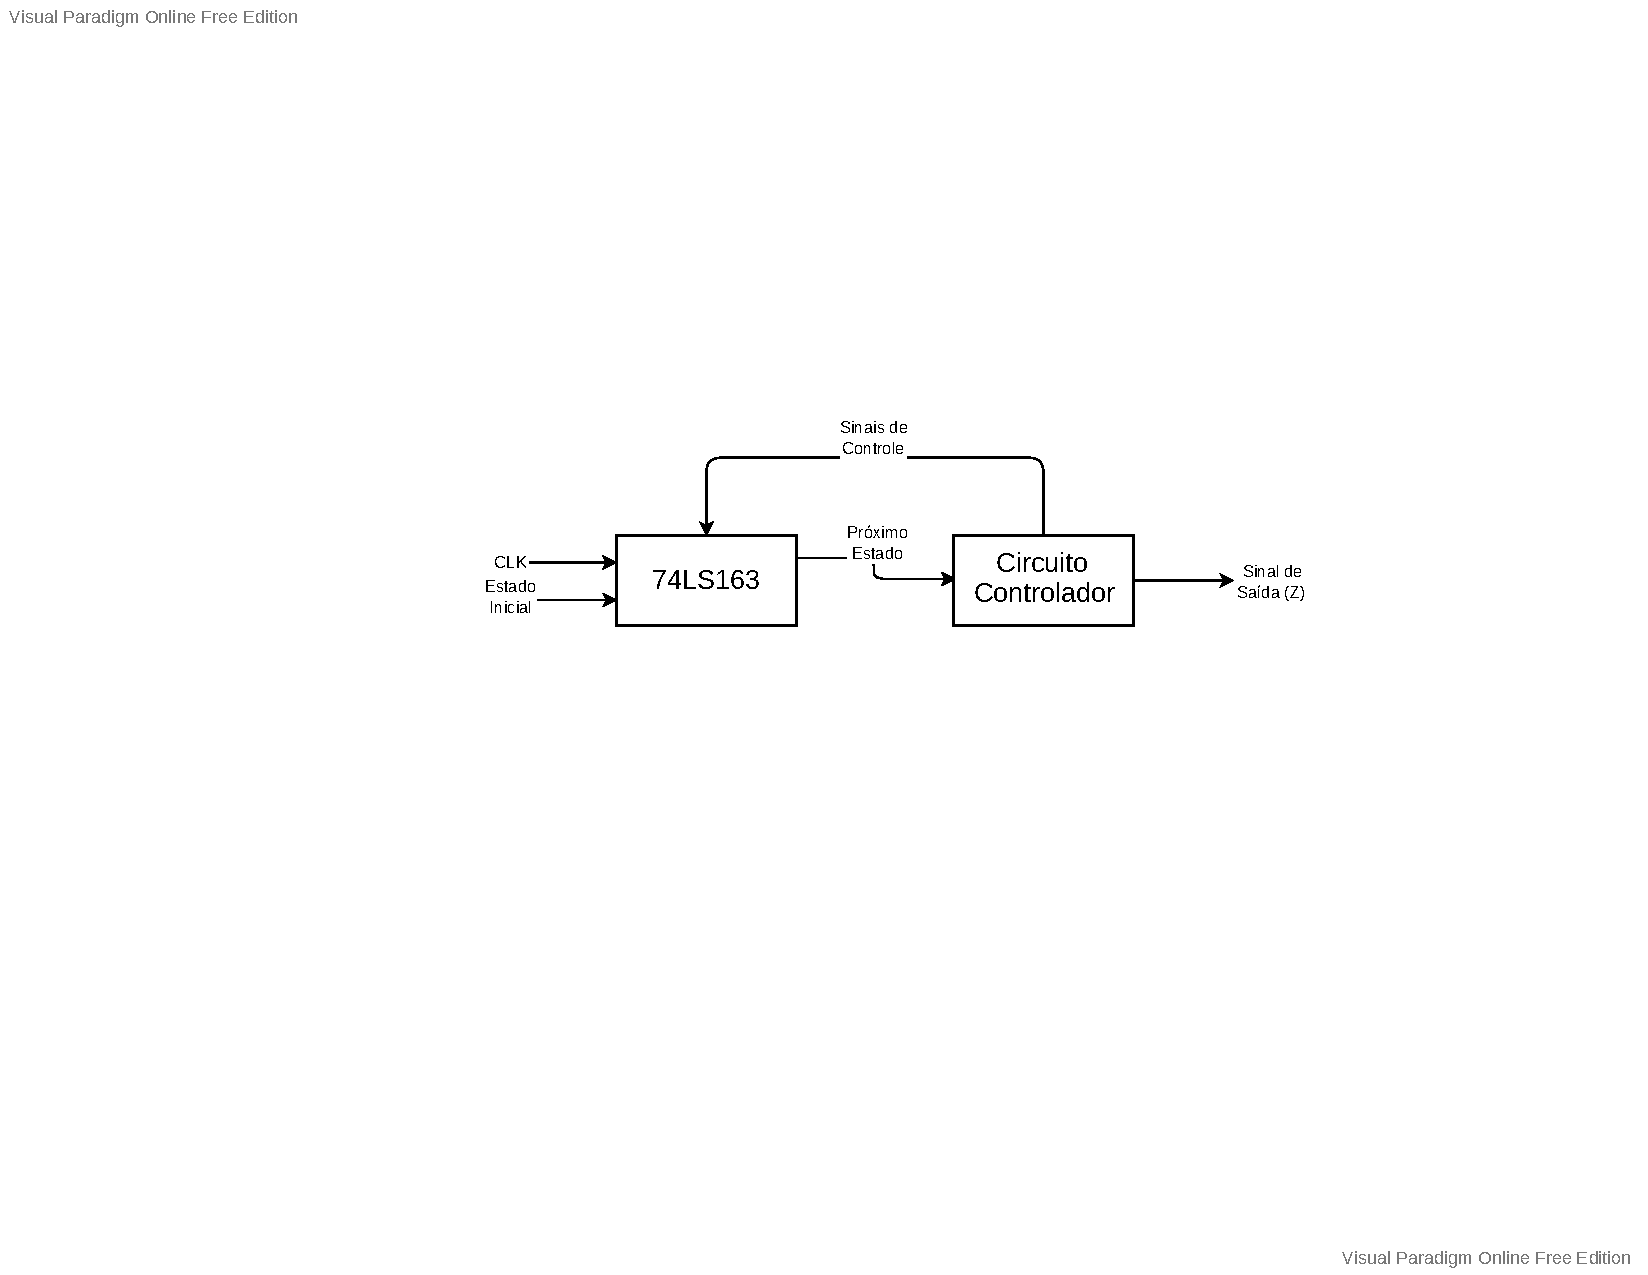
\includegraphics[width=0.81\textwidth, trim={75mm 90mm 55mm 60mm}, clip]{diagrama_blocos_74163.pdf}
  \caption{Diagrama de blocos do circuito contador síncrono usando o CI 74LS163}
  \label{fig:diagrama_blocos_74163}
\end{figure}

\subsubsection{Síntese do Circuito Controlador}
\label{sec:plan_74163_uc}

A síntese do circuito controlador constitui-se na construção de um circuito que desconsidera os estados 11, 12, 13, 14 e 15 do contador e vai do estado 10 direto para o estado zero, tal qual o diagrama de estados da Fig. \ref{fig:diagrama_estados_74163}.

\newpage
\begin{figure}[!ht]
  \centering
  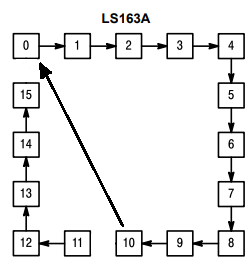
\includegraphics[width=0.36\textwidth]{diagrama_estados_74163.png}
  \caption{Diagrama de estados do 74LS163 com o circuito controlador desejado.}
  \label{fig:diagrama_estados_74163}
\end{figure}

Para isso, precisa-se analisar a Tabela \ref{tab:tb_verdade_74163} que mostra a lógica do circuito desejado. A coluna clk representa o sinal de entrada que é a borda de subida do clock, as colunas QD, QC, QB e QA são referentes às saídas do CI que representam o próximo estado, e as colunas Z, clr e load consistem na saída do circuito controlador. Os sinais clr e load retornarão para o CI enquanto o sinal Z já corresponde à saída do circutio como um todo. Nessa configuração, para o circuito retornar ao estado zero quando temos o sinal clr ou o sinal load iguais a zero, liga-se as 4 entradas de estado ao gnd. A partir desta tabela, é feito o mapa de Karnaugh para a saída Z do circuito controlador, tal como na Fig. \ref{fig:karnaugh_74163} no Apêndice \ref{ap:74163_karnaugh}. Com isso, obteve-se as seguintes expressões lógicas nas eqs. (\ref{eq:74163_Z}) e (\ref{eq:74163_clr_load}).

% \newpage
\begin{table}[!ht]
  \centering
  \caption{Tabela Verdade com os valore de saída para cada subida do clock e valores de saída do circuito controlador, que são os valores de Z, CLR e load}
  \label{tab:tb_verdade_74163}
  \doubleRuleSep
  \begin{tabular}{*{8}{c}}
    \doubleTopRule
    \multicolumn{1}{c}{Entrada} & \multicolumn{4}{c}{Saída 74LS163} & \multicolumn{3}{c}{Saída CC}                                                                \\
    \cmidrule(lr){1-1}\cmidrule(lr){2-5}\cmidrule(lr){6-8}
    clk                         & $QD$                              & $QC$                         & $QB$      & $QA$     & $Z$       & clr        & load         \\
    \midrule
    \csvreader[head to column names, late after line=\\]{tb_verdade_74163.csv}{}%
    {\csvcoli                   & \csvcolii                         & \csvcoliii                   & \csvcoliv & \csvcolv & \csvcolvi & \csvcolvii & \csvcolviii} %
    \doubleBottomRule
  \end{tabular}
\end{table}

\begin{align}
  Z   & = QD \cdot QC + QD \cdot QB\label{eq:74163_Z} \\
  clr & = load = \n{Z}\label{eq:74163_clr_load}
\end{align}

\subsubsection{Diagrama lógico}
\label{sec:plan_74163_logico}

A Fig. \ref{fig:diagrama_logico_74163} mostra o diagrama de lógico tanto do contador 74LS163 quanto do circuito de próximo estado, que é constituida de um circuito combinatório sintetizado a partir das eqs. (\ref{eq:74163_Z}) e (\ref{eq:74163_clr_load}).

% \newpage
\begin{figure}[!ht]
  \centering
  \stackinset{r}{1pt}{b}{1pt}{\carimboA{Contador 74LS163}}{%
    \stackinset{l}{1pt}{b}{1pt}{\carimboB{vcc3.csv}}{%
      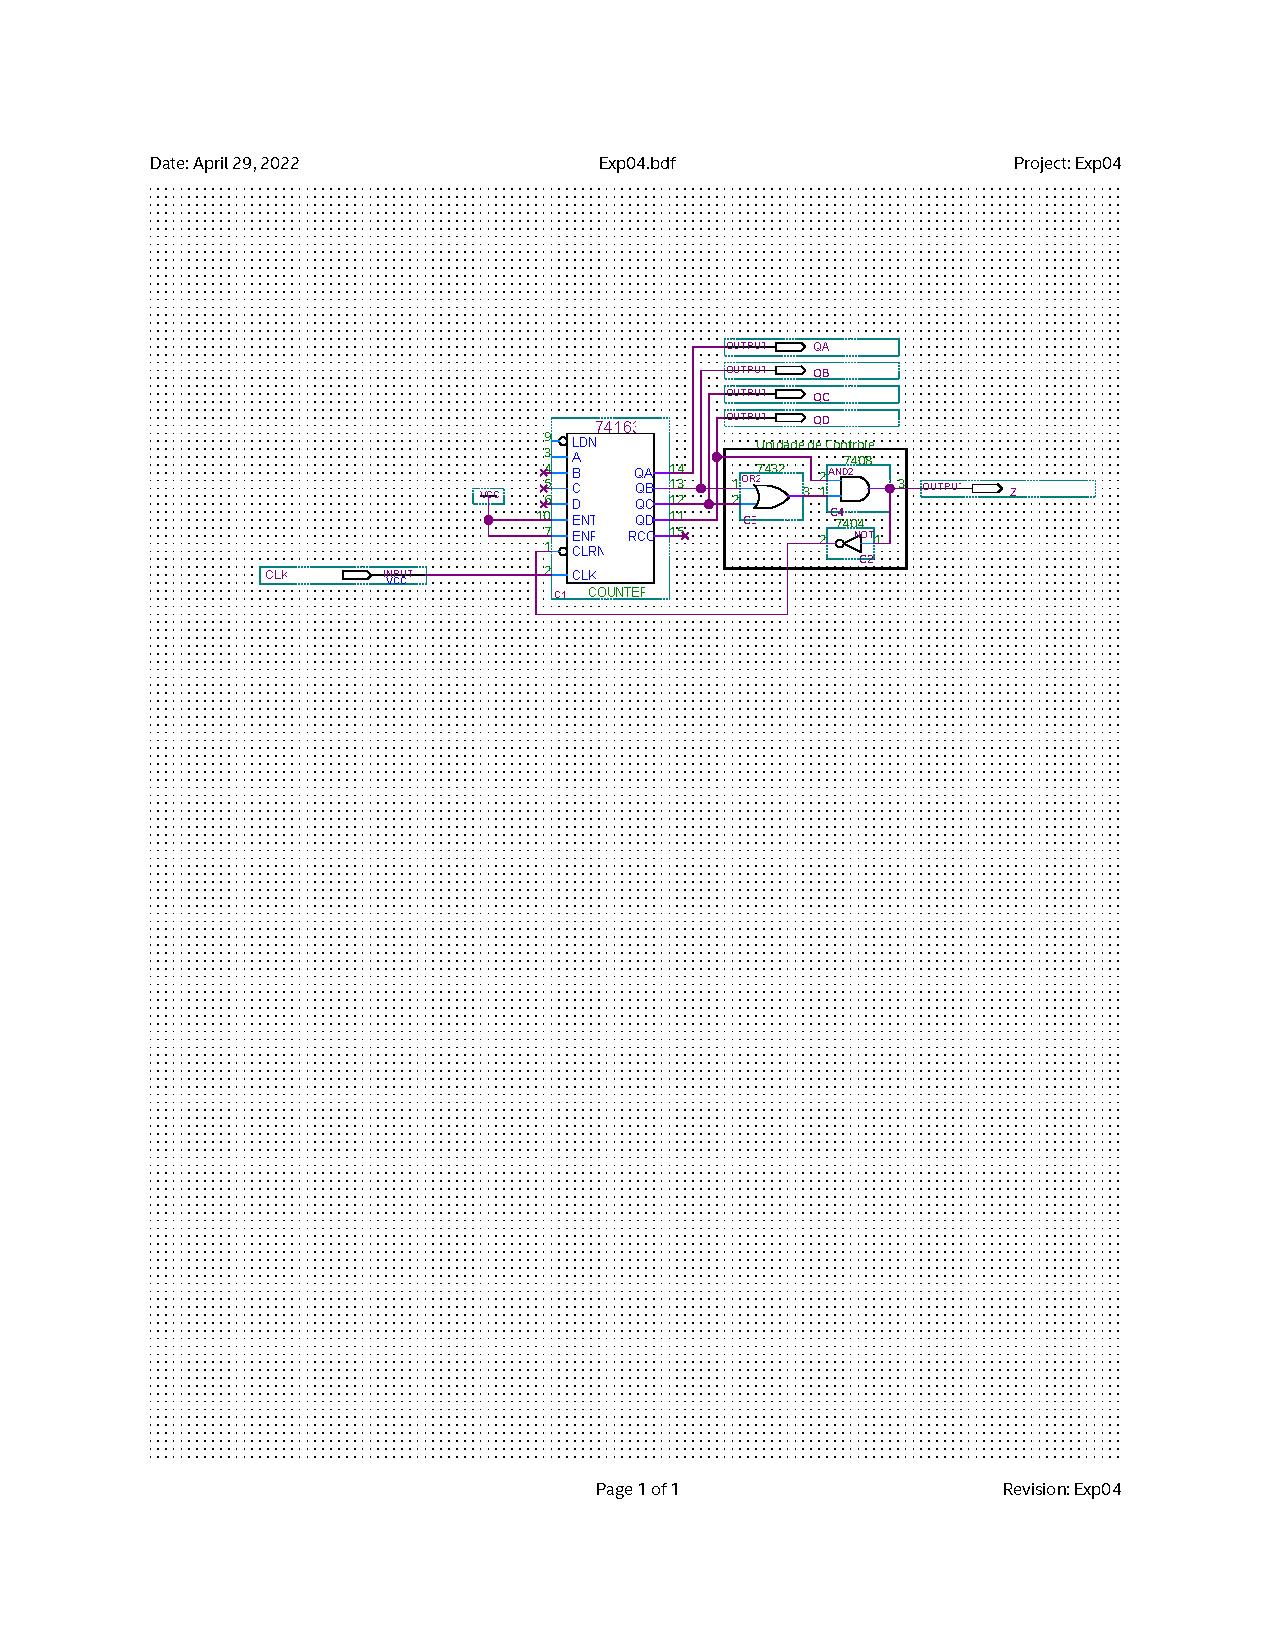
\includegraphics[width=\textwidth, trim={44mm, 164mm, 30mm, 55mm}, clip]{diagrama_74163_&_uc.pdf}%
    }%
  }
  \caption{Diagrama lógico do contador 74LS163 e do circuito controlador.}
  \label{fig:diagrama_logico_74163}
\end{figure}

\subsubsection{Levantamento dos materiais necessários}
\label{sec:plan_74163_levantamento}

\begin{table}[!ht]
  \centering
  \caption{Unidades requeridas para cada CI do projeto com o 74LS163}
  \label{tab:74163_materiais}
  \doubleRuleSep
  \begin{tabular}{lllrr}
    \doubleTopRule
    Slot & Operação & CI    & Un. Requeridas & Un. Disponíveis \\
    \midrule
    1    & Contador & 74163 & 1              & 1               \\
    2    & AND2     & 7408  & 1              & 4               \\
    3    & OR2      & 7432  & 1              & 4               \\
    4    & NOT      & 7404  & 1              & 6               \\
    \doubleBottomRule
  \end{tabular}
\end{table}

Para garantir que o circuito projetado respeite as restrições de montagem, fizemos um levantamento dos recursos necessários para este circuito mostrado na Tabela \ref{tab:74163_materiais}. Ela mostra a quantidade de unidades lógicas requeridas para cada CI utilizado. As especificações de cada CI foi obtido pelos respectivos \emph{datasheets}.

\subsubsection{Simulação}
\label{sec:plan_74163_simulacao}

A Fig. \ref{fig:carta_tempos_74163} mostra a carta dos tempos obtida com a simulação do contador. É possível notar que ela segue a tabela verdade descrita na Tabela \ref{tab:tb_verdade_74163} omitindo-se os sinais clr e load que na verdade são o sianl Z negado.

% \newpage
\begin{figure}[!ht]
  \centering
  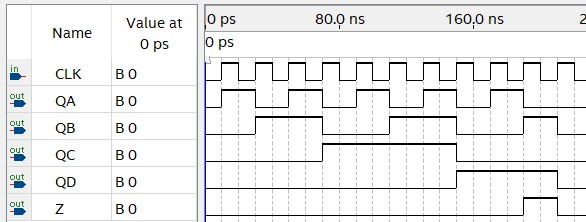
\includegraphics[width=\textwidth]{carta_tempos_74163.jpg}
  \caption{Carta dos tempos para o circuito contruído com o CI 74LS163 com sinial de entrada \texttt{clk}, sinais de depuração $QD$, $QC$, $QB$ e $QA$ (saídas do contador) e sinal de saída $Z$ (saída do Circuito Controlador)}
  \label{fig:carta_tempos_74163}
\end{figure}


\subsubsection{Metodologia de montagem e testes}
\label{sec:plan_74163_montagem}

O CI contador será testado juntamente com o circuito controlador, alterando manualmente o clock serão analisados tanto os sinais de saída do contador como o sinal de saída Z do circuito de próximo estado. O resultado será comparado com a Tabela \ref{tab:tb_verdade_74163}.

\section{Resultados}
\subsection{Contador módulo 11 utilizando flip-flops}
Antes da montagem, foi notado que as eqs. \eqref{eq:ff_d0} e \eqref{eq:ff_d2} poderiam ser simplificadas. A primeira colocando $\n{Q_0}$ em evidência e a segunda recalculando os mintermos e colocando $Q_2$ em evidência. Os mintermos da eq. \eqref{eq:ff_d2} não foram otimizados inicialmente intencionalmente devido à contagem de componentes da Tabela \ref{tab:ff_materiais}, mas, devido às mudanças, usamos a nova versão considerando todos os indeterminantes possíveis para reduzir o número de ligações. Assim, as eqs. \eqref{eq:ff2_d0}, \eqref{eq:ff2_d1}, \eqref{eq:ff2_d2} e \eqref{eq:ff2_d3} mostram as expressões usadas na montagem do circuito. As eqs. \eqref{eq:ff2_d1} e \eqref{eq:ff2_d3} permanencem inalteradas.

\begin{align}
  D_0 & = \n{Q_0}(\n{Q_1} + \n{Q_3})\label{eq:ff2_d0}                           \\
  D_1 & = \n{Q_1} \cdot Q_0 + \n{Q_3} \cdot Q_1 \cdot \n{Q_0}\label{eq:ff2_d1}  \\
  D_2 & = Q_2(\n{Q_1} + \n{Q_0}) + \n{Q_2} \cdot Q_1 \cdot Q_0\label{eq:ff2_d2} \\
  D_3 & = Q_3 \cdot \n{Q_1} + Q_2 \cdot Q_1 \cdot Q_0\label{eq:ff2_d3}
\end{align}

A montagem do circuito contator síncrono construído com flip-flops foi concluída, mas o valor obtido dos sinais não correspondeu ao valor esperado. A Tabela \ref{tab:tb_teste_ff} correlaciona os valores esperados com os obtinos. Em negrito é mostrado o dígito de saída do circuito de próximo estado que difere da tabela verdade. Essa divergência fez o circuito mudar para o estado 3 a partir do estado inicial. Então, partimos do sinal de saída de $D_1$ e checamos as ligações duas vezes, pois, se a montagem não representasse a expressão lógica de $D_1$, bastaria mudar as ligações, mas em ambas as vezes constatamos que as ligações feitas na placa de montagem representava a eq. \eqref{eq:ff2_d1}. E, como a expressão em questão foi a mesma simulada, então chegamos à conclusão de que o problema poderia ser do CI, mal contato, jumppers, etc.



\begin{table}[!ht]
  \centering
  \caption{Correlação entre os valores dos sinais de entrada, valores esperados e valores obtidos da saída dos flip-flops e da saída do circuito de próximo estado}
  \label{tab:tb_teste_ff}
  \doubleRuleSep
  \begin{tabular}{*{18}{c}}
    \doubleTopRule
    \multicolumn{2}{c}{}        & \multicolumn{8}{c}{Valores esperados} & \multicolumn{8}{c}{Valores obtidos}                                                                                                                                                                                                                                         \\
    \cmidrule(lr){3-10}\cmidrule(lr){11-18}
    \multicolumn{2}{c}{Entrada} & \multicolumn{4}{c}{Saída FF}          & \multicolumn{4}{c}{Saída CPE}       & \multicolumn{4}{c}{Saída FF} & \multicolumn{4}{c}{Saída CPE}                                                                                                                                                                          \\
    \cmidrule(lr){1-2}\cmidrule(lr){3-6}\cmidrule(lr){7-10}\cmidrule(lr){11-14}\cmidrule(lr){15-18}
    clk                         & clr                                   & $Q_3$                               & $Q_2$                        & $Q_1$                         & $Q_0$     & $D_3$      & $D_2$       & $D_1$     & $D_0$    & $Q_3$     & $Q_2$      & $Q_1$       & $Q_0$      & $D_3$     & $D_2$      & $D_1$       & $D_0$         \\
    \midrule
    \csvreader[head to column names, late after line=\\]{tb_teste_ff.csv}{}%
    {\csvcoli                   & \csvcolii                             & \csvcoliii                          & \csvcoliv                    & \csvcolv                      & \csvcolvi & \csvcolvii & \csvcolviii & \csvcolix & \csvcolx & \csvcolxi & \csvcolxii & \csvcolxiii & \csvcolxiv & \csvcolxv & \csvcolxvi & \csvcolxvii & \csvcolxviii} %
    \doubleBottomRule
  \end{tabular}
\end{table}


\subsection{Contador módulo 11 utilizando o CI 74LS613}
Nessa montagem, montou-se primeiramente o Circuito Controlador e testou-se a sua lógica utilizando as chaves do painel de montagem de modo que elas emulariam os sinais QD, QC e QB, tal qual na eq.(\ref{eq:74163_Z}), e um LED para o sinal Z. Logo em seguida conectou-se o circuito controlador ao CI 74LS163. Nessa segunda etapa da montagem, ligou-se os sinais QA, QB, QC e QD que saiam do 74163 aos LEDS, assim como a saída Z, e precionando um botão do painel de montagem simulou-se um pulso de cloque a cada precionada. Os resultados foram identicos aos esperado nessa montagem, tal qual pode ser observado na tabela a seguir.

\begin{table}[!ht]
  \centering
  \caption{Resultados obtidos após a montagem do circuito.}
  \label{tab:tb_testes_74163}
  \doubleRuleSep
  \begin{tabular}{*{8}{c}}
    \doubleTopRule
    \multicolumn{1}{c}{Entrada} & \multicolumn{4}{c}{Saída 74LS163} & \multicolumn{1}{c}{Saída CC}                                     \\
    \cmidrule(lr){1-1}\cmidrule(lr){2-5}\cmidrule(lr){6-6}
    clk                         & $QD$                              & $QC$                         & $QB$      & $QA$     & $Z$        \\
    \midrule
    \csvreader[head to column names, late after line=\\]{tb_teste_74163.csv}{}%
    {\csvcoli                   & \csvcolii                         & \csvcoliii                   & \csvcoliv & \csvcolv & \csvcolvi} %
    \doubleBottomRule
  \end{tabular}
\end{table}

As imagens da montagem do circuito se encontram no apêndice \ref{ap: 74163_montagem}.


\section{Conclusão}

Concluímos que é possível criar um circuito contador síncrono tanto a partir de flip-flops quanto a partir de CIs como 74163.


\newpage
\subsection*{Apêndice}
\appendix


\section{Material Suplementar do Contador FF}

\subsection{Mapas de Karnaugh do circuito de próximo estado}
\label{ap:ff_karnaugh}

\begin{figure}[!ht]
\centering
\begin{subfigure}[b]{0.49\textwidth}
\centering
\resizebox{.98\textwidth}{!}{%
  \begin{karnaugh-map}[4][4][1][$Q_1Q_0$][$Q_3Q_2$]
  \minterms{0,2,4,6,8}
  \indeterminants{12,13,14,15,11}
  \autoterms[0]
  \implicant{0}{8}
  \implicantedge{0}{4}{2}{6}
  \end{karnaugh-map}%
}
\caption{$D_0$}
\label{fig:karnaugh_ff_d0}
\end{subfigure}
\hfill
\begin{subfigure}[b]{0.49\textwidth}
\centering
\resizebox{.98\textwidth}{!}{%
  \begin{karnaugh-map}[4][4][1][$Q_1Q_0$][$Q_3Q_2$]
  \minterms{1,5,2,6,9}
  \indeterminants{12,13,14,15,11}
  \autoterms[0]
  \implicant{1}{9}
  \implicant{2}{6}
  \end{karnaugh-map}%
}
\caption{$D_1$}
\label{fig:karnaugh_ff_d1}
\end{subfigure}
\hfill\vspace{35pt}
\begin{subfigure}[b]{0.49\textwidth}
\centering
\resizebox{.98\textwidth}{!}{%
  \begin{karnaugh-map}[4][4][1][$Q_1Q_0$][$Q_3Q_2$]
  \minterms{3,4,5,6}
  \indeterminants{12,13,14,15,11}
  \autoterms[0]
  \implicant{3}{3}
  \implicant{4}{13}
  \implicant{6}{14}
  \end{karnaugh-map}%
}
\caption{$D_2$}
\label{fig:karnaugh_ff_d2}
\end{subfigure}
\hfill
\begin{subfigure}[b]{0.49\textwidth}
\centering
\resizebox{.98\textwidth}{!}{%
  \begin{karnaugh-map}[4][4][1][$Q_1Q_0$][$Q_3Q_2$]
  \minterms{7,8,9}
  \indeterminants{12,13,14,15,11}
  \autoterms[0]
  \implicant{12}{9}
  \implicant{7}{15}
  \end{karnaugh-map}%
}
\caption{$D_3$}
\label{fig:karnaugh_ff_d3}
\end{subfigure}
\caption{Mapas de Karnaugh para cada dígito da saída do circuito de próximo estado, que representa o próximo estado dos flip-flops}
\label{fig:karnaugh_ff}
\end{figure}

\section{Material Suplementar do Contador 74LS163}

\subsection{Mapa de Karnaugh do Circuito Controlador}
\label{ap:74163_karnaugh}

\begin{figure}[!ht]
\centering
\resizebox{0.5\textwidth}{!}{%
  \begin{karnaugh-map}[4][4][1][$Q_DQ_C$][$Q_BQ_A$]
  \minterms{3,7,10,11,14,15}
  \autoterms[0]
  \implicant{3}{11}
  \implicant{15}{10}
  \end{karnaugh-map}%
}
\caption{Mapa de Karnaugh do Circuito Controlador do circuito com o contador 74LS163}
\label{fig:karnaugh_74163}
\end{figure}

\subsection{Montagem do Contador módulo 11 utlizando o CI 74LS163}
\label{ap: 74163_montagem}

\begin{figure}[!ht]
  \centering
  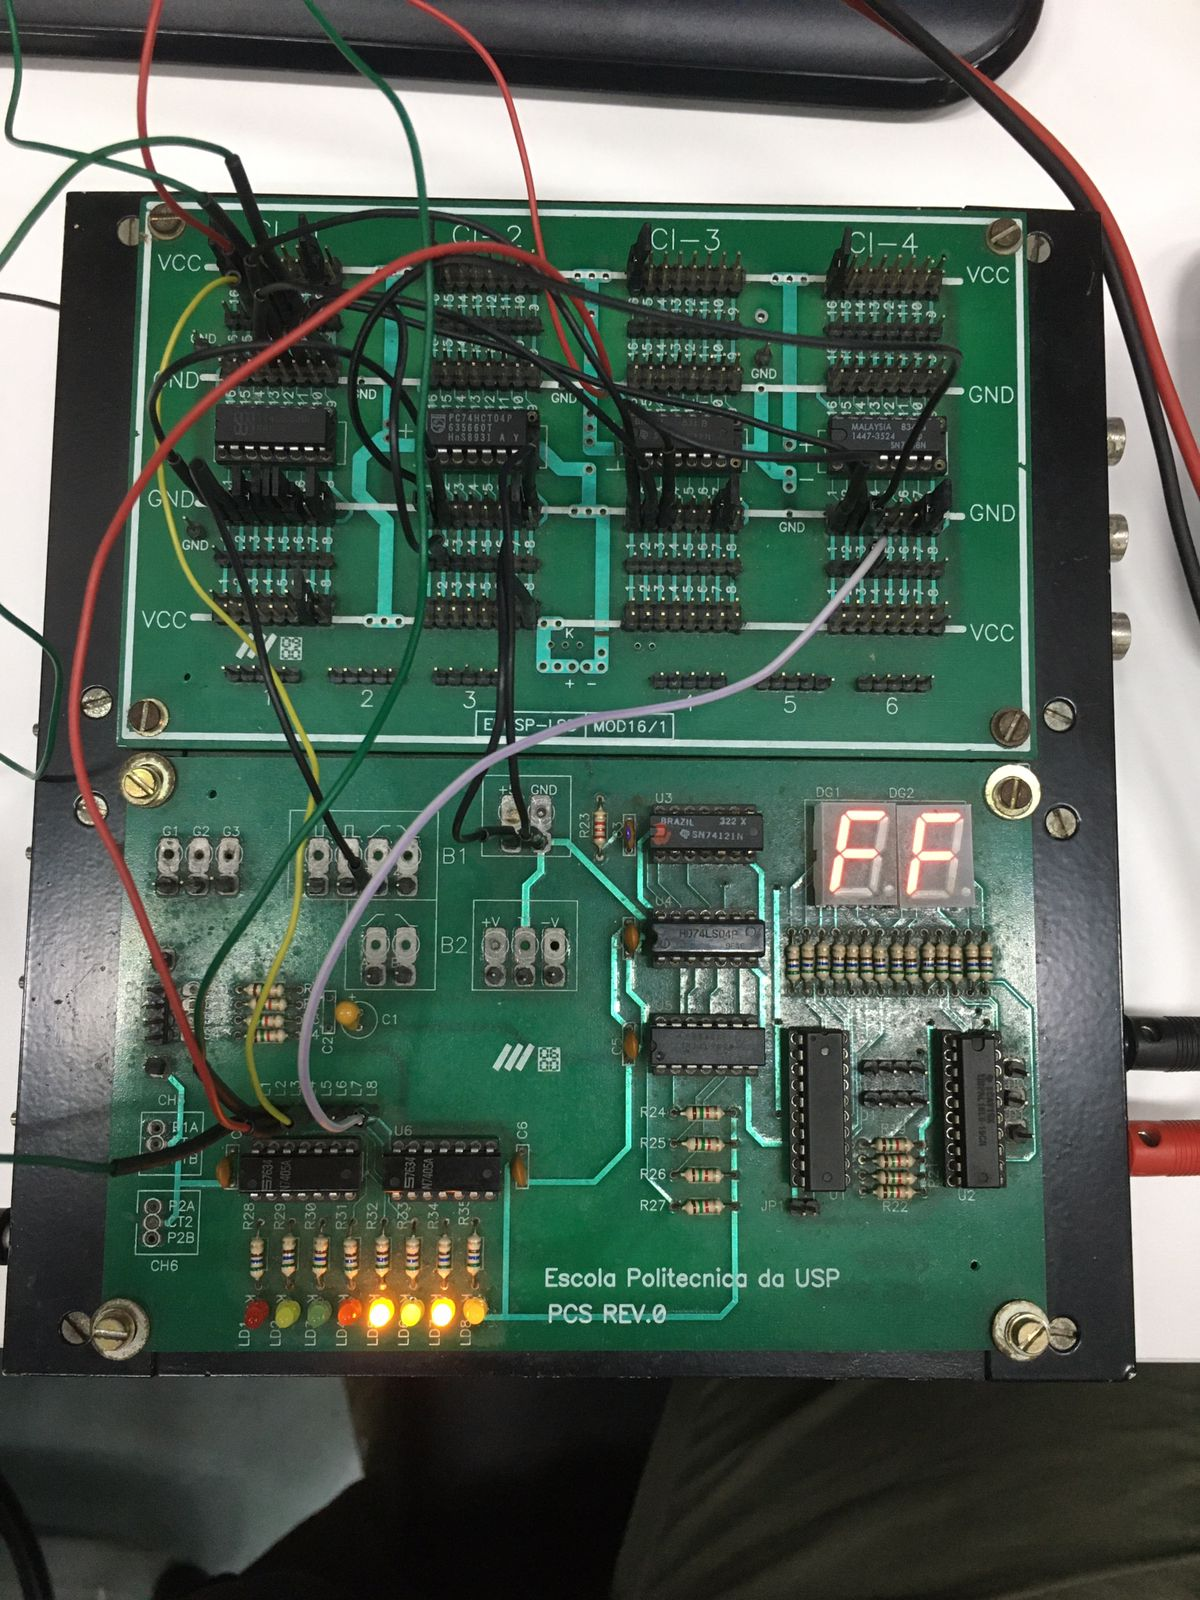
\includegraphics[width=0.36\textwidth, trim={30mm, 110mm, 40mm, 60mm}, clip]{74163_montagem.jpeg}
  \caption{Montagem do circuito contador módulo 11 com o CI 74LS163}
  \label{fig:montagem_74163}
\end{figure}

% \bibliographystyle{plainnat}
% \bibliography{refs}

\horizonBackCover
\end{document}
